\documentclass[11pt,a4paper]{article}
\author{TalentSprint}
\date{}
\usepackage{graphicx}
\usepackage{verbatim}
\usepackage{array}
\usepackage{caption}
\usepackage{enumitem}
\usepackage{xcolor}
\usepackage[tikz]{bclogo}
\usepackage{textcomp}
\usepackage{listings}
\usepackage{multicol}
\usepackage{float}
\usepackage{seqsplit} 
\usepackage{setspace}
\usepackage{soul}
\usepackage{latexsym}
\lstset{language=Java,numbers=left, numberstyle=\tiny, numbersep=10pt, showstringspaces=false, breaklines=true,keepspaces=true, columns=flexible}
\usepackage{fancyhdr}
\headheight=14pt
\lhead{\nouppercase{}}
\rhead{\nouppercase{\leftmark}}

\graphicspath{{../Images/}}


\begin{comment}
\setcounter{tocdepth}{1}
\setlength\parindent{0pt}
\parskip=4pt
\def\AnswerBox{\fbox{\begin{minipage}{4in}\hfill\vspace{0.5in}\end {minipage}}}

\thispagestyle{empty}
\vspace{1.5pc}
\topskip0pt
\vspace*{\fill}
\centerline{\sc \Huge Version Control System}
\vspace{2pc}
\vspace*{\fill}
\centerline{Prepared by TalentSprint WISE Team} 
\setcounter{page}{1}
\pagestyle{fancy}
\end{comment}


%========================================================================

% Lengths and widths
\addtolength{\textwidth}{2.5cm}
\addtolength{\hoffset}{0cm}
\setlength{\headsep}{-12pt} % Reduce space between header and content
\setlength{\headheight}{85pt} % If less, LaTeX automatically increases it
\renewcommand{\footrulewidth}{2pt} % Remove footer line
\renewcommand{\headrulewidth}{1pt} % Remove header line
\renewcommand{\seqinsert}{\ifmmode\allowbreak\else\-\fi} % Hyphens in seqsplit
% This two commands together give roughly
% the right line height in the tables
\renewcommand{\arraystretch}{1.3}
\onehalfspacing



% Commands
\newcommand{\SetRowColor}[1]{\noalign{\gdef\RowColorName{#1}}\rowcolor{\RowColorName}} % Shortcut for row colour
\newcommand{\mymulticolumn}[3]{\multicolumn{#1}{>{\columncolor{white}}#2}{#3}} % For coloured multi-cols
\newcolumntype{x}[1]{>{\raggedright}p{#1}} % New column types for ragged-right paragraph columns
\newcommand{\tn}{\tabularnewline} % Required as custom column type in use

% Font and Colours
\definecolor{HeadBackground}{HTML}{333333}
\definecolor{FootBackground}{HTML}{666666}
\definecolor{TextColor}{HTML}{333333}
\definecolor{DarkBackground}{HTML}{6B8E23} %{FD1AA8}
\definecolor{LightBackground}{HTML}{E8FED8} %D3FDC8
\definecolor{tit}{HTML}{FF6600}
\renewcommand{\familydefault}{\sfdefault}
\color{TextColor}
 \headsep = 25pt
% Header and Footer
\pagestyle{fancy}
\usepackage[headheight=110pt]{geometry}
\fancyhf{}% Clear header/footer

\fancyhead[r]{
\includegraphics[width = 4cm, height = 2cm]{TS-Logo.png}\hspace{0cm}}

%=================================TITLE=====================================
\fancyhead[l]{{\bf{\textcolor{tit}{\textrm{\large{JDBC}}}}}}
%===========================================================================

\renewcommand{\headrulewidth}{0.4pt}% Default \headrulewidth is 0.4pt
\renewcommand{\footrulewidth}{0.4pt}% Default \footrulewidth is 0pt

\rfoot{Page \thepage}
\lfoot{COPYRIGHT \textcopyright TALENTSPRINT, 2015. ALL RIGHTS RESERVED.}


\begin{document}

\section*{Introduction}
\texttt{JDBC} is an API (Application Programming Interface) that helps a programmer to write Java programs to connect to a database, retrieve the data from the database and perform various operations on the data in the Java program.

Every database vendor will provide a document representing all the commands to connect and utilize the database features. This document is called `API (Application Programming Interface) document'. API document is a file that contains description of all the features of a software, a product or a technology. The vendor of Oracle database has given functions like:
\begin{description} 
\item [oLog()] $\Longrightarrow$ to connect to database
\item [oexec()] $\Longrightarrow$ to execute a command
\item [oLogoff()] $\Longrightarrow$ to disconnect from Oracle database
\end{description}
In the same way MySQL database has give functions like: 
\begin{description}
\item [mysql\_connect()] $\Longrightarrow$ to connect to database
\item [mysql\_execute()] $\Longrightarrow$ to execute command
\item [mysql\_disconnect()] $\Longrightarrow$ to disconnect from MySQL database. 
\end{description}
This is cumbersome as there are hundereds of functions to learn. This is the reason software scientists have thought of creating a common API document. By using the functions of this common API document, programmers can communicate with any databse in the world, such document is called \texttt{ODBC} (Open Database Connectivity) API.

\texttt{ODBC} is a document that contains common functions to communicate with any database. It is created by Microsoft Corporation. If any organization creates a software depending on this ODBC document, it is called ODBC driver.

In the same way, Sun MicroSystems INC. has also created an API document named \texttt{JDBC} (Java Database Connectivity) API and the actual software which is created according to  \texttt{JDBC} API, is called \texttt{JDBC} Driver. \texttt{JDBC} API is defined in java.sql package. This package contains interfaces like \texttt{Connection, Statement, ResultSet, CallableStatement, Driver,}

\texttt{ResultSetMetaData, PreparedStatement} and classes like \texttt{Date, Time,}

\texttt{DriverManager} etc. Several companies have started developing software containing these interfaces and classes. These softwares are called JDBC drivers. For example, \textbf{classes12.jar} is a driver developed by Oracle corporation using which we can connect to Oracle database and communicate with it. Similarly \textbf{gate.jar} is a JDBC driver from inet to connect to Oracle. Similarly \textbf{Mysql-connector-java-3.0.11-stable-bin.jar} is a driver to connect to MySQL database. 

\section*{Stages in JDBC Program}
The following are the stages used by Java Programmers while using \texttt{JDBC} in their programs
\begin{enumerate}
\item \textbf{Registering the Driver:} database driver is a software containing classes and interfaces written according to \texttt{JDBC} API. Since there are several drivers avavailable in the market, we should first declare a driver which is going to be used for communication with the database server in a Java Program.
\item \textbf{Connecting to a database:} establish a connection with a specific database through the driver which is already registered.
\item \textbf{Preparing SQL statement in Java:} create SQL statements in our Java program using any of the interfaces like \texttt{Statement}, \\
\texttt{PreparedStatement} which are available in java.sql package.
\item \textbf{Executing the SQL statements on the database:} \texttt{execute(), executeQuery()} and \texttt{executeUpdate()} methods of Statement interface are used to execute \texttt{SQL} statements.
\item \textbf{Retrieving the results:} obtained by executing the SQL statements can be stored in an object with the help of interfaces like \texttt{ResultSet, ResultSetMetaData} and \texttt{DatabaseMetaData}.
\item \textbf{Closing the connection:} close the connection between the Java program and the database by using \texttt{close()} method of \texttt{Connection} interface.
\end{enumerate}

\subsection*{Registering the Driver}
This is the first step to connect to a database. A programmer should specify which database driver can be used to connect to the database. There are different ways to register a driver.
\begin{enumerate}
    \item By creating an object to driver class of the driver software. For example to register mysql driver, create an object to the driver class as shown below

\lstinline!com.mysql.jdbc.Driver = new com.mysql.jdbc.Driver();!
 \item By sending the driver class object to \texttt{registerDriver()} method of \texttt{DriverManager} class. For example, the object of mysql can be passed to registerDriver method as

\lstinline!DriverManager.registerDriver(``com.mysql.jdbc.Driver'');!
 \item By sending the driver class name directly to \texttt{forName()} method as

 \lstinline!Class.forName(``com.mysql.jdbc.Driver'');!
\end{enumerate}
 \subsection*{Connecting to Database}
 To connect to database, we should know three things
 \begin{description}
\item[URL of the database] URL (Uniform Resource Locator) represents a protocol to connect to the database. Simply speaking it locates the database on the network.
\item[Username] to connect to the database, every user will be given a username which is generally alloted by the database administrator.
\item[Password] is the password alloted to the user by the database administrator to connect to the database.
\end{description}
For Example, to connect to mysql database, write the following statement.
\begin{lstlisting}[numbers=none]
DriverManager.getConnection
(``jdbc:mysql://localhost/test'', ``root'', ``root'');
\end{lstlisting}
Here, ``jdbc:mysql://localhost/test'' is the URL, ``root'' is the username, ``root'' is the password.
\begin{description}
\item[Example] Program to connect to the Database.
\lstinputlisting{../Code/ConnectionExample.java}
\end{description}

\subsection*{Preparing and Executing SQL Statements}
We need \texttt{SQL} (Structured Query Language) statements which are useful to make different operations like creating table in the database, adding data to the database, updating the data of the database, deleting the data from the database and also retrieving the data from the database. SQL statements can be classified into two types as follows.
\begin{description}
    \item[select statements] help to retrieve data from the database in the form of rows.
    \item[non-select statements] represents all other statements except select statement like create, update, delete etc.
\end{description}

The Statement interface provides three methods for creating SQL queries and returning a result.
\begin{description}
\item[boolean execute(sqlstring)] returns a boolean indicating if \texttt{ResultSet} was returned. Many SQL statements can be executed with execute.
\item[int executeUpdate(sqlstring)] returns an int (number of rows affected) or 0 when the statement is a \texttt{Data Defination Statement (DDL) statement}, such as \texttt{CREATE TABLE}.
\item[ResultSet executeQuery(sqlstring)] returns a \texttt{ResultSet} object.
\end{description}
For Example, to create a table Student, we can use create statement as:
\begin{lstlisting}[numbers=none]
CREATE TABLE Student(sid int(32), 
sname Varchar(35), age int(32), 
address Varchar(50))
\end{lstlisting}
To execute the above statement, create statement object, as
\begin{lstlisting}[numbers=none]
Statement stmt = con.createStatement();
\end{lstlisting}
And then, pass the SQL statement to \texttt{execute()} method as
\begin{lstlisting}[numbers=none]
stmt.execute(``CREATE TABLE Student(sid int(32),
sname Varchar(35), age int(32), 
address Varchar(50))'');
 \end{lstlisting}

\begin{description}
\item[Example] Program to create table.
\lstinputlisting{../Code/CreateTableExample.java}
\end{description}
\begin{description}
\item[Example] Program to insert records.
\lstinputlisting{../Code/InsertRecordsExample.java}
\end{description}

\subsection*{Closing Connection}
After executing all the required SQL statements and obtaining the results, close the connection and release the session. This can be done by calling \texttt{close()} method of the \texttt{Connection} interface as follows.
\begin{lstlisting}[numbers=none]
Connection.close();
\end{lstlisting}
\begin{description}
\item[Example] Program to Insert records.
\lstinputlisting{../Code/InsertCloseExample.java}
\end{description}
\vfill{\ }
\begin{figure}[H]
 \begin{center}
   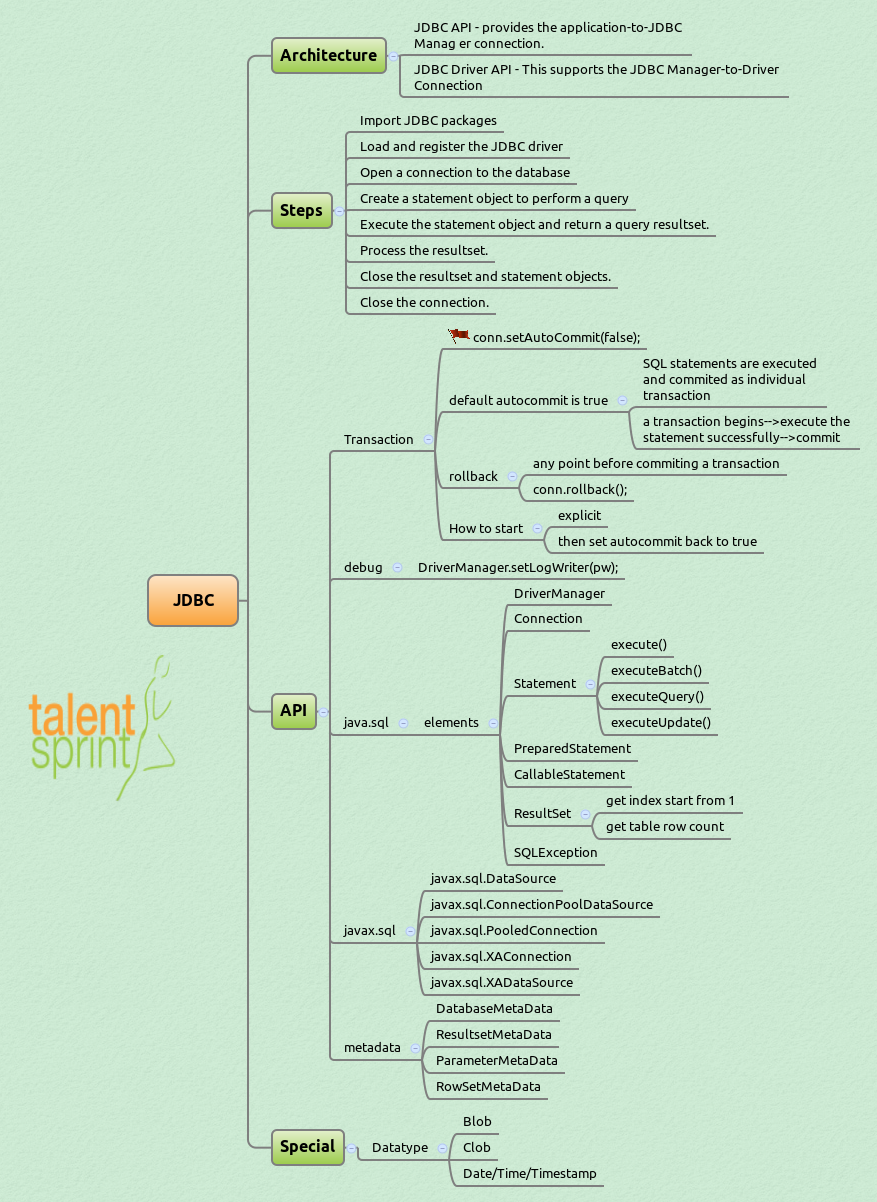
\includegraphics[angle=90,height=20cm, width=13cm]{JDBC.png}
 \end{center}
 \end{figure}
\section*{PreparedStatement}
Using \texttt{PreparedStatement} in place of \texttt{Statement} interface will improve the performance of a JDBC program. When a SQL statement is sent to database, the following tasks are performed
\begin{itemize}
\item The SQL statement's syntax should be verified to know whether it is correct or not. The SQL statement is divided into small pieces called \texttt{`tokens'}. These tokens are also verified to know whether they are in \texttt{SQL} format or not.
\item The another verification is done to know whether the table mentioned in the statement exists or not.
 \end{itemize}
The above two statements are called \texttt{`parsing'} and takes some time. When a SQL statement is executed, \texttt{Statement} interfcae does parsing every time the statement is executed and takes more time. On the other hand, if we use \texttt{PreparedStatement}, it does parsing only once and saves time. Hence \texttt{PreparedStatement} offers better performance.

We should create \texttt{PreparedStatement} object using \texttt{prepareStatement()} method of \texttt{Connection} interface as

\begin{lstlisting}[numbers=none]
PreparedStatement stmt = con.prepareStatement(``INSERT 
INTO Student VALUES(?, ?, ?, ?)'');
\end{lstlisting}
Here, \texttt{`?'} represents the value to be passed to the columns of the row. The first \texttt{?} represents the value to be passed to the first column and the second \texttt{?} represents the value for second column. These values can be passed using \texttt{setXXX()} method as
\begin{lstlisting}[numbers=none]
setInt(1, value);
setString(2, value);
\end{lstlisting}

\begin{description}
\item[Example] Program to insert records using PreparedStatement.
\lstinputlisting{../Code/PsInsertExample.java}
\end{description}
\section*{Working With ResultSet Interface}
\texttt{ResultSet} is an interface that manages the resulting data returned from a \texttt{Statement}.

\subsection*{ResultSet objects}
\begin{itemize}
    \item \texttt{ResultSet} maintains a cursor to the returned rows. The cursor is initially pointing before the first row.
    \item The \texttt{ResultSet.next()} method is called to position the cursor in the next row.
    \item The default \texttt{ResultSet} is not updatable and has a cursor that points only forward.
    \item It is possible to produce \texttt{ResultSet} objects that are scrollable and/or updatable as follows.
\end{itemize}
\begin{lstlisting}[numbers=none]
Statement stmt = con.createStatement
                 (ResultSet.TYPE_SCROLL_INSENSITIVE,  
                  ResultSet.CONCUR_UPDATABLE);
\end{lstlisting}

\subsection*{ResultSet methods}
\begin{description}
\item[boolean next()] moves the cursor to the one row next from the current position.
\item[boolean previous()] moves the cursor to the one row previous from the current position.
\item[boolean first()] moves the cursor to the first row in result set object.
\item[boolean last()] moves the cursor to the last row in result set object.
\item[boolean absolute(int row)] moves the cursor to the specified row number in the ResultSet object.
\item[boolean relative(int row)] moves the cursor to the relative row number in the ResultSet object, it may be positive or negative.
\item[int getInt(int columnIndex)] returns the data of specified column index of the current row as int.
\item[int getInt(String columnName)] returns the data of specified column name of the current row as int.
\item[String getString(int columnIndex)] returns the data of specified column index of the current row as String.
\item[String getString(String columnName)] returns the data of specified column name of the current row as String.
\end{description}

\begin{description}
\item[Example] Program to retrieve records.
\lstinputlisting{../Code/SelectExample.java}
\end{description}

\subsection*{ResultSetMetaData Interface}
\texttt{ResultSetMetaData} interface is used to describe a JDBC Driver object that encapsulates the metadata of the cursor. The \texttt{ResultSetMetaData} object is used to retrieve information about the columns in a \texttt{ResultSet}. It can also be used to get the information like column names, column datatypes, and column length, related to particular result. The \texttt{ResultSetMetaData} object is obtained by using the \texttt{ResultSet} object, that is by invoking the \texttt{getMetaData()} method on the \texttt{ResultSet} object.

\subsubsection*{Methods of ResultSetMetaData}
\begin{description}
    \item[getColumnCount()] returns an integer value and retrieves the number of columns in the \texttt{ResultSet} object.
    \item[getColumnName(int index)] takes the column index and returns the column name.
    \item[getColumnType(int index)] takes the column index and returns the integer value that indicates the columns SQL type.
    \item[getColumnLabel(int index)] retrieves the title of the specified column in the \texttt{ResultSet} object.
    \item[getTableName(int column)] retrieves the name of the specified column in the \texttt{ResultSet} object.
    \item[getColumnTypeName(int index)] takes the column index and returns the database specific type name.
\end{description}


\begin{description}
     \item[Example] Program to demonstrate ResultSetMetaData.
         \lstinputlisting{../Code/RSMetaDataExample.java}
 \end{description}


\section*{Working With Batch Updates}
The batch update option allows you to submit multiple Data Manipulation Language (DML) operations to a database as a single unit. Submitting multiple DML statements together, rather than submitting them individually, improves the performance of the system by reducing the time consumption in executing statements.

\subsection*{Batch Update Methods}
\begin{description}
    \item[addBatch(String SQLStatement)] adds the given SQL statement to the current batch i.e, the batch that is managed by this \texttt{Statement} object.
    \item[clearBatch()] clears the batch currently assosiated with this Statement object.
    \item[int\lbrack\rbrack executeBatch()] submits the current batch on this \texttt{Statement} object to the underlying datasource. Once the batch is submitted to the data source, the statements in a batch are executed in the sequence in which thay have been added to the batch. The following are the outcomes of this method.
        \begin{itemize}
            \item If the batch executes successfully, this method returns an array of integer values whose length is equal to the number of statements in the batch.
            \item If the value of any element in this array is equal to STATEMENT.SUCCESS\_NO\_INFO, it indicates that the statement has been executed successfully but the number of rows affected is unknown.
            \item In case a statement in a batch fails to be executed or produces a result set , further processing of the batch execution depends on the database that is in use. The database may continue to execute the batch or may terminate it.
        \end{itemize}
\end{description}


\begin{description}
\item[Example] Program to demonstrate Batch Updates.
\lstinputlisting{../Code/BatchExample.java}
\end{description}

\section*{DataBaseMetaData Interface}
\texttt{DataBaseMetaData} is an interface implemented by the JDBC driver provider. The \texttt{DataBaseMetaData} object encapsulates all the information related to the database and driver. The \texttt{DataBaseMetaData} object is useful to get the database details, such as DB vendor name, product name, version etc. Use the \texttt{Connection.getMetaData()} method to get the \texttt{DataBaseMetaData} object.

\subsection*{Methods of DataBaseMetaData}
\begin{description}
    \item[int getDataBaseMajorVersion()] retrieves the major version number of the database in use.
    \item[int getDataBaseMinorVersion()] retrieves the minor version number of the database in use.
    \item[String getDataBaseProductName()] retrieves the name of this database product.
    \item[String getDataBaseProductVersion()] retrieves the version number of this database product.
    \item[int getDriverMajorVersion()] retrieves the major version number of the JDBC Driver.
    \item[int getDriverMinorVersion()] retrieves the minor version number of the JDBC Driver.
    \item[int getMaxRowSize()] retrieves the maximum number of bytes a database allows in a single row.
    \item[int getMaxConnections()] retreives the maximun number of concurrent connections to a database that are possible.
    \item[String getDriverName()] retrieves the name of this JDBC driver.
    \item[String getURL()] retrieves the URL for this DBMS.
    \item[String getUserName()] retrieves the user name as known to this database.
\end{description}

\begin{description}
    \item[Example] Program to demonstrate DataBaseMetaData.
    \lstinputlisting{../Code/DBMetaDataExample.java}
\end{description}

\section*{Transactions}
\texttt{Transaction} is a set of statements executed on a resource or resources applying ACID properties. In multiple environments various users work on databases and there may be chances of data loss. Therefore, to avoid data loss, DBMS is used to maintain data integrity within database. \texttt{Transactions} are required to provide data integrity, correct application semantics, and a consistent view of data during concurent acess. In general, DBMS provides \texttt{atomicity, consistency, isolation,} and \texttt{durability} for each transaction in a database. These properties are collectively called as the \texttt{ACID} properties.

\subsection*{Describing ACID properties}
\begin{description}
    \item[Atomicity] is the ability of a transaction to hold the decision of saving the statement until the end of the set of statements i.e, transactions.
    \item[Consistency] guarantees that the data remains in a legal state when the transaction begins and ends.
    \item[Isolation] is the ability of the transaction to isolate or hide the data from other transactions until it ends.
    \item[Durability] guarantees that once the user has been notified of the successful transaction i.e, if a transaction is commited , it will persist all the statements or it will leave complete transaction unsaved.
\end{description}
\subsection*{JDBC Transactions}
By default, when a Connection is created, transaction is in auto-commit mode.
\begin{itemize}
\item Each individual SQL statement is treated as transaction and automatically commited after it is executed.
\item To group two or more statements together, disable auto-commit mode.
\begin{lstlisting}[numbers=none]
Connection.setAutoCommit(false);
\end{lstlisting}
\item Explicitly call the commit method to complete the transaction with in the database.
\begin{lstlisting}[numbers=none]
Connection.commit();
\end{lstlisting}
\item Transactions can be rollbacked programatically in the event of failure.
\begin{lstlisting}[numbers=none]
Connection.rollback();
\end{lstlisting}
  \end{itemize}

By default, JDBC auto commits all SQL statements. However when you want to create an atomic operations that involves multiple SQL statements, disable auto-commit. After auto-commit is disabled no SQL statements are commited to the database until commit method is called explicitly. The other advantage of managing transactions is the ability to rollback the set of statements in the event of failure using rollback method.
\begin{bclogo}[couleur=blue!5, arrondi=0.3]{Note}
Create table and Insert the data as given below in the database.


CREATE TABLE Bank(accno int, bal int);

INSERT INTO Bank VALUES(101, 10000);

INSERT INTO Bank VALUES(102, 10000);
\end{bclogo}

\begin{description}
\item[Example] Program to demonstrate Transactions.
\lstinputlisting{../Code/TransactionExample.java}
\end{description}

\end{document}